\documentclass[final,12pt]{colt2018} % Anonymized submission
%\documentclass[anon,12pt]{colt2018} % Include author names


% The following packages will be automatically loaded:
% amsmath, amssymb, natbib, graphicx, url, algorithm2e
% use Times
\usepackage{times}
\usepackage[font=small,skip=0pt]{caption}


% For figures
\usepackage{graphicx} % more modern
%\usepackage{epsfig} % less modern
%\usepackage{caption}
%\usepackage{subcaption}
%\usepackage{subfigure}
\usepackage{footnote}
\makesavenoteenv{tabular}
\makesavenoteenv{table}
% For citations
%\usepackage{natbib}
\usepackage{amsmath}
%\usepackage{amsthm}
\usepackage{amssymb}
\usepackage{tikz}
\usepackage{xcolor}
\usetikzlibrary{arrows}
\usepackage{hyperref}
\usepackage{enumerate}

% For algorithms
\usepackage{algorithm}
\usepackage{algorithmic}
\usepackage{hyperref}
\usepackage{bm}
\usepackage{footnote}
\newcommand*\samethanks[1][\value{footnote}]{\footnotemark[#1]}

\newcommand\blfootnote[1]{%
	\begingroup
	\renewcommand\thefootnote{}\footnote{#1}%
	\addtocounter{footnote}{-1}%
	\endgroup
}

%For theorems

\usepackage{varwidth}
%for convinience
\newcommand{\vct}{\boldsymbol }
%\newcommand{\mat}{\mathbf}
\newcommand{\rnd}{\mathsf}
\newcommand{\ud}{\mathrm d}
\newcommand{\nml}{\mathcal{N}}
\newcommand{\loss}{\mathcal{L}}
\newcommand{\hinge}{\mathcal{R}}
\newcommand{\kl}{\mathrm{KL}}
\newcommand{\cov}{\mathrm{cov}}
\newcommand{\dir}{\mathrm{Dir}}
\newcommand{\mult}{\mathrm{Mult}}
\newcommand{\err}{\mathrm{err}}
\newcommand{\sgn}{\mathrm{sgn}}
%\renewcommand{\span}{\mathrm{span}}
\newcommand{\argmin}{\mathrm{argmin}}
\newcommand{\argmax}{\mathrm{argmax}}
\newcommand{\poly}{\mathrm{poly}}
\newcommand{\rank}{\mathrm{rank}}
\newcommand{\conv}{\mathrm{conv}}
\newcommand{\E}{\mathbb{E}}
\newcommand{\diag}{\mat{diag}}
\newcommand{\acc}{\mathrm{acc}}
\newcommand{\polylog}{\mathrm{polylog}}

\newcommand{\aff}{\mathrm{aff}}
\newcommand{\range}{\mathrm{Range}}
\newcommand{\Sgn}{\mathrm{sign}}

\newcommand{\hit}{\mathrm{hit}}
\newcommand{\cross}{\mathrm{cross}}
\newcommand{\Left}{\mathrm{left}}
\newcommand{\Right}{\mathrm{right}}
\newcommand{\Mid}{\mathrm{mid}}
\newcommand{\bern}{\mathrm{Bernoulli}}
\newcommand{\ols}{\mathrm{ols}}
\newcommand{\tr}{\mathrm{tr}}
\newcommand{\opt}{\mathrm{opt}}
\newcommand{\ridge}{\mathrm{ridge}}
\newcommand{\unif}{\mathrm{unif}}
\newcommand{\Image}{\mathrm{im}}
\newcommand{\Kernel}{\mathrm{ker}}
\newcommand{\supp}{\mathrm{supp}}
\newcommand{\pred}{\mathrm{pred}}
\newcommand{\goodind}{\mathcal{G}}
\newcommand{\badind}{\mathcal{B}}
\newcommand{\func}{g}
\newcommand{\meandiff}{\Delta}
\newcommand{\covdiff}{\mathcal{E}}
\newcommand{\lip}{L}
\newcommand{\op}{\mathrm{op}}
\newcommand{\expect}{\mathbb{E}}
\newcommand{\holder}{H\"{o}lder }
\newcommand{\ind}{1}


\newenvironment{proofof}[1]
{
 \par\noindent{\bfseries\upshape Proof of #1\ }%
 }%
 {\jmlrQED}
 
 \newenvironment{proofsketchof}[1]
 {
 	\par\noindent{\bfseries\upshape Proof Sketch of #1\ }%
 }%
 {\jmlrQED}
 
 
 \newenvironment{proofsketch}
 {
 	\par\noindent{\bfseries\upshape Proof Sketch\ }%
 }%
 {\jmlrQED}
 
 \renewcommand{\algorithmicrequire}{\textbf{Input:}} 
 \renewcommand{\algorithmicensure}{\textbf{Output:}}



\def\R{\mathbb{R}}
\def\Z{\mathbb{Z}}
\def\N{\mathbb{N}}
\def\cA{\mathcal{A}}
\def\cB{\mathcal{B}}
\def\cC{\mathcal{C}}
\def\cD{\mathcal{D}}
\def\cE{\mathcal{E}}
\def\cF{\mathcal{F}}
\def\cG{\mathcal{G}}
\def\cH{\mathcal{H}}
\def\cI{\mathcal{I}}
\def\cL{\mathcal{L}}
\def\cM{\mathcal{M}}
\def\cN{\mathcal{N}}
\def\cP{\mathcal{P}}
\def\cS{\mathcal{S}}
\def\cT{\mathcal{T}}
\def\cW{\mathcal{W}}
\def\cX{\mathcal{X}}
\def\cY{\mathcal{Y}}
\def\cZ{\mathcal{Z}}
\def\bP{\mathbf{P}}
\def\TV{\mathrm{TV}}
\def\MSE{\mathrm{MSE}}

\newcommand{\mat}[1]{{#1}}
%\newcommand{\set}[1]{{#1}}
\newcommand{\vect}[1]{\mathrm{vec}\left({#1}\right)}
\newcommand{\norm}[1]{\left\|#1\right\|}
\newcommand{\abs}[1]{\left|#1\right|}
%\newcommand{\expect}[1]{\mathbf{E}\left[#1\right]}
\newcommand{\prob}{\mathbb{P}}
\newcommand{\prox}[2]{\textbf{Prox}_{#1}\left\{#2\right\}}
\newcommand{\tops}{P_{2k}}
\newcommand{\nodiag}{P}


\newtheorem{thm}{Theorem}[section]
%\newtheorem{lem}{Lemma}[section]
\newtheorem{lem}[thm]{Lemma}
\newtheorem{cor}[thm]{Corollary}
\newtheorem{claim}[thm]{Claim}
\newtheorem{prop}[thm]{Proposition}
\newtheorem{assumption}[thm]{Assumption}
\newtheorem{defn}[thm]{Definition}
\newtheorem{fact}[thm]{Fact}
\newtheorem{conj}[thm]{Conjecture}
\newtheorem{rem}[thm]{Remark}
\newtheorem*{remark*}{Remark}

% Siva's macros
\newcommand{\samplesize}{n}
\newcommand{\fronorm}[1]{\ensuremath{\matsnorm{#1}{\footnotesize{\mbox{F}}}}}
\newcommand{\opnorm}[1]{\ensuremath{\matsnorm{#1}{\footnotesize{\mbox{op}}}}}
\newcommand{\matnorm}[3]{|\!|\!| #1 | \! | \!|_{{#2}, {#3}}}
\newcommand{\matsnorm}[2]{\left|\!\left|\!\left|#1\right|\!\right|\!\right|_{{#2}}}
\newcommand{\vecnorm}[2]{\| #1\|_{#2}}
\newcommand{\inprod}[2]{\ensuremath{\langle #1 , \, #2 \rangle}}
\newcommand{\sparseopnorm}[1]{\ensuremath{\matsnorm{#1}{\footnotesize{\mbox{k,op}}}}}

%Jerry
\newcommand{\new}[1]{{\color{red} #1}}
\newcommand{\X}{\mathcal{X}}
\newcommand{\W}{\mathcal{W}}
\newcommand{\Xt}{{\mathcal{Z}}}
\newcommand{\Sgood}{\mathcal{G}}
\newcommand{\Sbad}{\mathcal{B}}
\newcommand{\Sigmahat}{\widehat{\Sigma}}


\newcommand{\dx}{\mathrm{d}x}
\newcommand{\seteq}{\mathrel{\mathop:}=}

\DeclareMathOperator{\diam}{\mathsf{Diam}}


%for comments

\newcommand{\Pnote}[1]{{[\color{blue}P: #1]}}
\newcommand{\wei}[1]{\textsf{\color{red}[Wei: #1]}}
\newcommand{\sanjeev}[1]{\textsf{\color{green}[Sanjeev: #1]}}

\newcommand{\Id}{I}
\newcommand{\KL}{\text{KL}}
\renewcommand{\conv}{\mathsf{Conv}}

\allowdisplaybreaks


\title{An Analysis of the t-SNE Algorithm for Data Visualization}



  % Authors with different addresses:
 \coltauthor{\Name{Sanjeev Arora} \Email{arora@cs.princeton.edu}\\
 	\addr Princeton University
 	\AND
 	\Name{Wei Hu} \Email{huwei@cs.princeton.edu}\\
 	\addr Princeton University
 	\AND
 	\Name{Pravesh K. Kothari} \Email{kothari@cs.princeton.edu}\\
 	\addr Princeton University \& Institute for Advanced Study
 }


\begin{document}
%\let\thefootnote\relax\footnote{some text}
%\addtocounter{footnote}{-1}\let\thefootnote\svthefootnote
\blfootnote{Extended abstract. Full version appears as \hyperref{https://arxiv.org/abs/1803.01768}{}{}{arXiv:1803.01768}.}

\maketitle
\begin{abstract}%\label{sec:abs}
We present preconditioned stochastic gradient descent (SGD) algorithms for the $\ell_1$ minimization problem $\min_{\xx}\|\AA \xx - \bb\|_1$ in the overdetermined case, where there are far more constraints than variables. Specifically, we have $\AA \in \R^{n \times d}$ for $n \gg d$. Commonly known as the Least Absolute Deviations problem, $\ell_1$ regression can be used to solve many important combinatorial problems, such as minimum cut and shortest path. SGD-based algorithms are appealing for their simplicity and practical efficiency.
% Our algorithms precondition the matrix $\AA$ and then solve the problem for the resulting matrix $\tilde{\AA}$ using gradient descent techniques.
Our primary insight is that careful preprocessing can yield preconditioned matrices $\tilde{\AA}$ with strong properties (besides good condition number and low-dimension) that allow for faster convergence of gradient descent. In particular, we precondition using Lewis weights to obtain an isotropic matrix with fewer rows and strong upper bounds on all row norms. We leverage these conditions to find a good initialization, which we use along with recent smoothing reductions and accelerated stochastic gradient descent algorithms to achieve $\epsilon$ relative error in $\Otil(nnz(\AA) + d^{2.5} \epsilon^{-2})$ time with high probability, where $nnz(\AA)$ is the number of non-zeros in $\AA$. This improves over the previous best result using gradient descent for $\ell_1$ regression. We also match the best known running times for interior point methods in several settings.

Finally, we also show that if our original matrix $\AA$ is approximately isotropic and the row norms are approximately equal, we can give an algorithm that avoids using fast matrix multiplication and obtains a running time of $\Otil(nnz(\AA) + s d^{1.5}\epsilon^{-2} + d^2\epsilon^{-2})$, where $s$ is the maximum number of non-zeros in a row of $\AA$. In this setting, we beat the best interior point methods for certain parameter regimes.


%We consider the $\ell_1$ minimization problem $\min_{\xx}||\AA \xx - \bb||_1$ in the overconstrained case, where there are far more constraints than variables. More specifically, we have $\AA \in \R^{n \times d}$ for $n \gg d$. By using Lewis Weights preconditioning on $\AA$ and a careful initialization, we show that a standard stochastic gradient descent algorithm achieves $\epsilon$ relative error in about $nnz(\AA) +  d^3\epsilon^{-2}$ time with high probability. If we leverage smoothing reductions in \cite{AllenZhuH16} and the accelerated stochastic gradient descent algorithms in \cite{AllenZhu17}, we can achieve a running time of about $nnz(\AA) + d^{2.5}\epsilon^{-2}$ with the same guarantees. Both of these running times improve over the previous results in \cite{YangCRM16} and the latter result is comparable to the best known running times for interior point methods \cite{LeeS15}.
%
%The key idea will be to use our preconditioning to restrict our consideration to matrices $\AA$ such that $\AA^T\AA = \II$ and every row norm of $\AA$ is upper bounded by $O(\sqrt{d/n})$. \cite{cohenpeng} show that sampling $\AA$ with Lewis weights takes about $nnz(\AA) +d^{\omega}$ time and approximately preserves the minimization problem. Moreover, we can assume $n\le O(d\epsilon^{-2}\log n)$ for the sampled matrix. We then prove that all leverage scores of the sampled matrix are approximately equal. Since rotations preserve leverage scores, we can then rotate our sampled matrix to ensure that our desired properties are met in about $d^{\omega}\epsilon^{-2}$ time.
%
%Finally, we also show that if our original matrix $\AA$ is such that $\AA^T\AA \approx \II$ and the row norms of $\AA$ are bounded, we can avoid using fast matrix multiplication and prove a running time of about $nnz(\AA) + s d^{1.5}\epsilon^{-2}$, where $s$ is the maximum number of non-zeros in a row of $\AA$.

%Consequently, we will be able to restrict our consideration to matrices $A$ such that $A^TA \approx I$, and all row norms are equal, which is to say $||A_{i,:}||_2 = \sqrt{\frac{d}{n}}$ for all $i$.
%
%With a careful choice of our initial $x$, we show that standard gradient descent and stochastic gradient descent algorithms under these further assumptions only require $O(\frac{d}{\epsilon^2})$ and $O(\frac{d^2}{\epsilon^2})$ iterations, respectively, to achieve $\epsilon$ relative error with respect to the minimum objective value. Accordingly, these methods each achieve respective total runtime of $O(\frac{md}{\epsilon^2})$ and $O(\frac{d^3}{\epsilon^2})$, along with an $O(m)$ preconditioning cost, improving over the previous results in \cite{MahoneySGD}.
%
%We further examine the consequences of our assumptions when combined with smoothing reductions in [cite] and accelerated gradient descent techniques in [cite,cite]. As a result we are able to further improve the running times to $O(\frac{md}{\epsilon})$ and $O(dn\log{1/\epsilon} + \frac{d^2\sqrt{n}}{\epsilon})$.
%
%Random sampling $d\epsilon^{-2}\log{d}$ rows of $A$ will only incur error $\epsilon$ and reduces the latter running time to $O(\frac{d^{2.5}\log{d}}{\epsilon^2})$, which is then comparable to interior point methods of [cite]

\end{abstract}

\begin{keywords}
Clustering, t-SNE, Visualization	
\end{keywords}

% !TeX root = main.tex
\section{Introduction}
\label{sec:intro}
Generative models are often trained in an unsupervised fashion, fitting a model $q$ to a set of observed data $x_P \subseteq X$ drawn iid from some true distribution $p$ on $x\in X$. Now, of course $p$ may not exactly belong to family $Q$ of probability distributions being fit, whether $Q$ consists of Gaussians mixture models, Markov models, or even neural networks of bounded size. We first discuss the limitations of generative modeling without feedback, and then discuss our model and results.

%\subsection{Limitations of Generative Modeling from Positive Examples Alone}
Consider fitting a generative model on a text corpus consisting partly of poetry written by four-year-olds and partly of mathematical publications from the {\em Annals of Mathematics}. Suppose that learning to generate a poem that looks like it was written by a child was easier than learning to generate a novel mathematical article with a correct, nontrivial statement. If the generative model pays a high price for generating unrealistic examples, then it may be better off learning to generate children's poetry than mathematical publications. However, without negative feedback, it may be difficult for a neural network or any other model to know that the mathematical articles it is generating are stylistically similar to the mathematical publications but do not contain valid proofs.\footnote{This is excluding clearly fake articles published without proper review in lower-tier venues \citep{LabbeL13}.} 

As a simpler example, the classic Markovian ``trigram model'' of natural language assigns each word a fixed probability conditioned only on the previous two words. Prior to recent advances in deep learning, for decades the trigram model and its variant were the workhorses of language modeling, assigning much greater likelihood to natural language corpora than numerous linguistically motivated grammars and other attempts \citep{Rosenfeld00}. However, text sampled from a trigram is typically nonsensical, e.g., the following text was randomly generated from a trigram model fit on a corpus of text from the Wall Street Journal \citep{JurafskyM09}:
\begin{quote}
They also point to ninety nine point six billion dollars from two hundred
four oh six three percent of the rates of interest stores as Mexico and
gram Brazil on market conditions. 
\end{quote}

In some applications, like text compression using a language model \citep{WittenNC87}, maximizing likelihood is equivalent to optimizing compression. However, in many  applications involving generation, such nonsense is costly and unacceptable. Now, of course it is possible to always generate valid data by returning random training examples, but this is simply overfitting and not learning. Alternatively, one could incorporate human-in-the-loop feedback such as through crowdsourcing, into the generative model to determine what is a valid, plausible sentence.

In some domains, validity could be determined automatically. Consider a Markovian model of a well-defined concept such as mathematical formulas that compile in \LaTeX{}. Now, consider a $n$-gram Markovian character model which the probability of each subsequent character is determined by the previous $n$ characters. For instance, the expression \$\{2+\{x-y\}\$ is invalid in \LaTeX{} due to mismatched braces. For this problem, a \LaTeX{} compiler may serve as a validity oracle. Various $n$-gram models can be fit which only generate valid formulas. To address mismatched braces, for example, one such model would ensure that it always closed braces within $n$ characters of opening, and had no nested braces. While an $n$-gram model will not perfectly model the true distribution over valid \LaTeX{} formulas, for certain generative purposes one may prefer an $n$-gram model that generates valid formulas over one that assigns greater likelihood to the training data but generates invalid formulas. 

Figure \ref{fig:rectangle} illustrates a simple case of learning a rectangle model for data which is not uniform over a rectangle. A maximum likelihood model would necessarily be the smallest rectangle containing all the data, but most examples generated from this distribution may be invalid. Instead a smaller rectangle, as illustrated in the figure, may be desired.

\begin{figure}[h]\label{fig:rectangle}
\centering
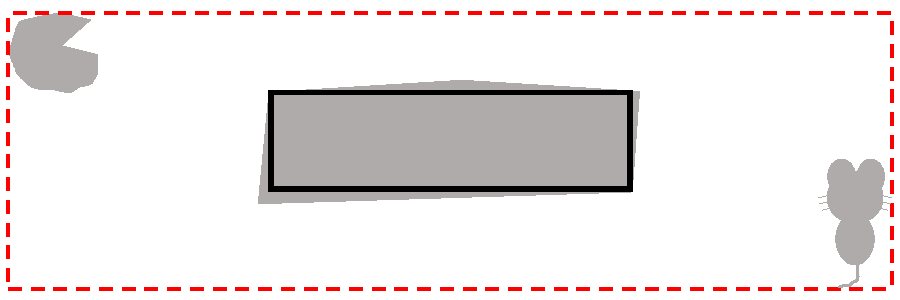
\includegraphics[width=3in]{fig.pdf}
\caption{Example where the underlying distribution $p$ is uniform over the (gray) valid regions. The solid rectangle maximizes our objective since it does not output nonsense (is supported only within the grey matter) and is closest to the $p$ (covers the maximum amount of grey matter). In contrast, the standard maximum likelihood (dashed red) rectangle must fully contain the observed samples, thus generating invalid points most of the time.  }
\end{figure}

Motivated by these observations, we evaluate a generative model $q$ on two axes. First is {\em coverage}, which is related to the probability assigned to future examples drawn from the true distribution $p$. Second is {\em validity}, defined as the probability that random examples generated from $q$ meet some validity requirement. Formally, we measure coverage in terms of a bounded {\em loss}:
$$\Loss(p,q)=\E_{x \sim p}[L(q_x)],$$
where $L:[0,1]\rightarrow [0,M]$ is a bounded decreasing function such as the capped log-loss $L(q_x)=\min(M, \log 1/q_x)$. % or $L(q_x)=\log 1/(q_x+\exp(-M))$. 
A bounded loss has the advantages of being efficiently estimable, and also it enables a model to assign 0 probability to one example (e.g., an outlier or error) if it greatly increases the likelihood of all other data. Validity is defined with respect to a set $V \subseteq X$, and $q(V)$ is the probability that a random example generated from $q$ lies within $V$. 

Clearly, there is a tradeoff between coverage and validity. We first focus on the case of (near) perfect validity. A Valid Generative Modeling (VGM) algorithm if it outputs, for a family of distributions $Q$ over $X$, if it outputs $\hat{q}$ with (nearly) perfect validity and whose loss is nearly as good as the loss of the best valid $q\in Q$. More precisely, $A$ is a VGM learner of $Q$ if for any nonempty valid subset $V \subseteq X$, any probability distribution $p$ over $V$, and any $\eps>0$, $A$ uses $n$ random samples from $p$ and makes $m$ membership oracle calls to $V$ and outputs a distribution $\hat{q}$ such that, $$\Loss(p, \hat{q}) \leq \min_{q \in Q: q(V)=1}\Loss(p,q) + \eps ~\text{ and }~\hat{q}(V)\geq 1-\eps.$$ 
We aim for our learner to be sample and query efficient, requiring that $n$ and $m$ are polynomial in $M, 1/\eps$ and a measure of complexity of our distribution class $Q$.
Furthermore, we would like our algorithms to be computationally efficient, with a runtime polynomial in the size of the data, namely the $n + m$ training examples. 
A more formal description of the problem is available in Section~\ref{sec:problem}.

$A$ is said to be {\em proper} if it always outputs $\hat{q}\in Q$ and {\em improper} otherwise.
In Section~\ref{sec:impossibility}, we first show that efficient proper learning for VGM is impossible. This is an information-theoretic result, meaning that even given infinite runtime and positive samples, one still cannot solve the VGM problem. Interestingly, this is different from binary classification, where it is possible to statistically learn from iid examples without a membership oracle.

Our first main positive result is an efficient (improper) learner for VGM. The algorithm relies on a subroutine that solves the following {\em Generative Modeling with Negatives} (GMN) problem: given sets $X_P, X_N \subset X$ of positive and negative examples, find the probability distribution $q \in Q$ which minimizes $\sum_{x \in X_P} L(q(x))$ subject to the constraint that $q(X_N)=0$. For simplicity, we present our algorithm for the case that the distribution family $Q$ is finite, giving sample and query complexity bounds that are logarithmic in terms of $|Q|$. However, as we show in Section~\ref{sec:infinite-families}, all of our results extend to infinite families $Q$. It follows that if one has a computationally efficient algorithm for the GMN problem for a distribution family $Q$, then our reduction gives a computationally efficient VGM learning algorithm for $Q$.

Our second positive result is an algorithm that minimizes $\Loss(p,q)$ subject to a relaxed validity constraint comparing against the optimal distribution that has validity $q(V)$ at least $1-\alpha$ for some $\alpha>0$. We show in Section~\ref{sec:partial-validity} that even in this more general setting, it is possible to obtain an algorithm that is statistically efficient but may not be computationally efficient. An important open question is whether there exists a computationally efficient algorithm for this problem when given access to an optimization oracle, as was the case for our algorithm for VGM.

\subsection{Related Work}
\cite{KearnsMRRSS94} showed how to learn distributions from positive examples in the realizable setting, i.e., where the true distribution is assumed to belong to the class being learned. In the same sense as their work is similar to PAC learning \citet{Valiant84} of distributions, our work is like agnostic learning \citet{KearnsSS94} in which no assumption on the true distribution is made. 

Generative Adversarial Networks (GANs)~\cite{GoodfellowPMXWOCB14} are an approach for generative modeling from positive examples alone, in which a generative model is trained against a discriminator that aims to distinguish real data from generated data. In some domains, GANs have been shown to outperform other methods at generating realistic-looking examples. Several shortcomings of GANs have been observed \citet{AroraRZ18}, and GANs are still subject to the theoretical limitations we argue are inherent to any model trained without a validity oracle. 

In supervised learning, there is a rich history of learning theory with various types of queries, including membership which are not unlike our (in)validity oracle. Under various assumptions, queries have been shown to facilitate the learning of complex classes such as finite automata \citet{Angluin88} and DNFs \citet{Jackson97}. See the survey of \cite{Angluin92} for further details.  Interestingly, \cite{Feldman09} has shown that for agnostic learning, i.e., without making assumptions on the generating distribution, the addition of membership queries does not enhance what is learnable beyond random examples alone. 
Supervised learning also has a large literature around active learning, showing how the ability to query examples reduces the sample complexity of many algorithms. See the survey of \cite{Hanneke14}. Note that the aim here is typically to save examples and not to expand what is learnable.
 
More sophisticated models, e.g., involving neural networks, can mitigate the invalidity problem as they often generate more realistic natural language and have even been demonstrated to generate \LaTeX{} that nearly compiles \citep{Karpathy15} or nearly valid Wikipedia markdown. However, longer strings generated are unlikely to be valid. For example, \cite{Karpathy15} shows generated markdown which includes:
\begin{quote}
==Access to ''rap===
The current history of the BGA has been [[Vatican Oriolean Diet]], British Armenian, published in 1893.  While actualistic such conditions such as the [[Style Mark Romanians]] are still nearly not the loss.
\end{quote}

Even ignoring the mismatched quotes and equal signs, note that this example has two so-called ``red links'' to two pages that do not exist. Without checking, it was not obvious to us whether or not Wikipedia had pages titled {\em Vatican Oriolean Diet} or {\em Style Mark Romanians}. In some applications, one may or may not want to disallow red links. In the case that they are considered valid, one may seek a full generative model of what might plausibly occur inside of brackets, as the neural network has learned in this case. If they are disallowed, a model might memorize links it has seen but not generate new ones. A validity oracle can help the learner identify what it should avoid generating.

 In practice, \cite{KusnerPH17} discuss how generative models from neural networks (in particular autoencoders) often generate invalid sequences. 
\cite{JanzWPKH18} learn the validity of examples output by a generative model using oracle feedback. 

%!TEX root = main.tex


\subsection{Related Work}
This paper continues the line of work focused on analyzing gradient descent and related heuristics for non-convex optimization problems, examples of which we have discussed before. Theoretically analyzing t-SNE, in particular, was recently considered in a work of \citet{linderman2017clustering} who showed that running t-SNE with early exaggeration causes points from the same cluster to move towards each other (i.e., embedding of any cluster shrinks). As discussed before, however, this does not imply that t-SNE ends up with a visualization as all the clusters could potentially collapse into each other.
Another work by \cite{shaham2017stochastic} derived a theoretical property of SNE, but their result is only nontrivial when the number of clusters is significantly larger than the number of points per cluster, which is an unrealistic assumption.


Mixture models are natural average-case generative models for clusterable data which have been studied as benchmarks for analyzing various clustering algorithms and have a long history of theoretical work. By now, a sequence of results~\citep{DBLP:conf/soda/DasguptaHKM07,DBLP:conf/esa/DasguptaHKM06,arora2005learning,vempala2004spectral,DBLP:conf/colt/AchlioptasM05,DBLP:conf/colt/KannanSV05,DBLP:conf/colt/Vempala07,MR3385380-Hsu13,DBLP:conf/stoc/GeHK15,DBLP:journals/cacm/KalaiMV12,DBLP:conf/focs/BelkinS10,DBLP:conf/stoc/KalaiMV10,DBLP:journals/corr/abs-1711-07465,DBLP:journals/corr/abs-1711-07454,DBLP:journals/corr/abs-1711-07211} have identified efficient algorithms for clustering data from such models under various natural assumptions. %Mixtures of log-concave distributions have also been studied in a similar context~\citep{}.

%%!TEX root = main.tex

\section{Preliminaries}
In this section, we will review some well-known results on~\gd~and~\nag~in the strongly convex setting, 
and existing results on convergence of~\gd~to second-order stationary points. 
% The pseudocode for these algorithms is given in Algorithms~\ref{algo:gd} and~\ref{algo:AGD} respectively.

% \cnote{Show gradient descent in equation}

\subsection{Notation}
Bold upper-case letters ($\A, \B$) denote matrices and bold lower-case letters ($\x, \y$) denote vectors. 
For vectors $\norm{\cdot}$ denotes the $\ell_2$-norm. For matrices, $\norm{\cdot}$ denotes the spectral norm and $\lambda_{\min}(\cdot)$ denotes the minimum eigenvalue.
For $f: \R^d \rightarrow \R$, $\grad f(\cdot)$ and  $\hess f(\cdot)$ denote its gradient and Hessian respectively, and $f^\star$ denotes its global minimum.
% Other than Section \ref{sec:related}, 
We use $O(\cdot), \Theta(\cdot), \Omega(\cdot)$ to hide absolute constants, and $\tilde{O}(\cdot), \tilde{\Theta}(\cdot), \tilde{\Omega}(\cdot)$ to hide absolute constants and polylog factors for all problem parameters. 
% \praneeth{I think it will be cleaner to make the dependence on smoothness parameters in Table~\ref{tab:main} and edit this statement} \jccomment{Then I also need to add function value dependence, maybe too complicated to compare}.\praneeth{The issue with this is that $O()$ is not just hiding constants but also problem dependent parameters. May be mention this explicitly in the caption to the table.} 
% We let $\ball^{(d)}_\x(r)$ denote the d-dimensional ball centered at $\x$ with radius $r$; when it is clear from context, we simply denote it as $\ball_\x(r)$. We use $\proj_{\mathcal{X}}(\cdot)$ to denote projection onto the set $\mathcal{X}$. Distance and projection are always defined in a Euclidean sense.


% \pn{Talk about ignoring $\log d$ factors in notation.}

\subsection{Convex Setting}\label{sec:prelim_convex}
% \begin{figure}[t]
% \begin{minipage}{0.5\textwidth}
% 	\begin{algorithm}[H]
% 	\caption{\gd($\x_0, \eta$)}\label{algo:gd}
% 	\begin{algorithmic}[1]
% 		\For{$t = 0, 1, \ldots, T $}
% 		\State $\x_{t+1} \leftarrow \x_t - \eta \grad f (\x_t)$
% 		\EndFor
% 		\State \textbf{return} $\x_T$
% 	\end{algorithmic}
% 	\end{algorithm}
% 	\vspace{0.5cm}
% \end{minipage}
% \begin{minipage}{.5\textwidth}

% \end{minipage}
% \end{figure}
To minimize a function $f(\cdot)$,~\gd ~performs the following sequence of steps:
\begin{equation*}
\x_{t+1} = \x_{t}- \eta \grad f(\x_t).
\end{equation*}
The suboptimality of~\gd~and the improvement achieved by~\nag~can be clearly illustrated for the case of smooth and strongly convex functions. %The definitions of smoothness and strong convexity are as follows.
\begin{definition}\label{def:smooth}
A differentiable function $f(\cdot)$ is \textbf{$\ell$-smooth (or $\ell$-gradient Lipschitz)} if:
\begin{equation*}
\norm{\grad f(\x_1) - \grad f(\x_2)} \le \ell \norm{\x_1 - \x_2} \quad \forall \; \x_1, \x_2.
\end{equation*}
\end{definition}
\noindent
The gradient Lipschitz property asserts that the gradient can not change too rapidly in a small local region.
\begin{definition}\label{def:convex}
A twice-differentiable function $f(\cdot)$ is \textbf{$\alpha$-strongly convex} if
$\lambda_{\min}(\hess f(\x)) \ge \alpha, \;  \forall \; \x$.
% $f(\x_2) \ge f(\x_1) + \la \grad f(\x_1), \x_2 - \x_1 \ra + \frac{\alpha}{2}\norm{\x_2 - \x_1}^2, \quad \forall \; \x_1, \x_2.$
\end{definition}
Let $\fstar \defeq \min_{\y}f(\y)$. A point $\x$ is said to be \textbf{$\epsilon$-suboptimal} if $f(\x)  \le  \fstar + \epsilon$. The following theorem gives the convergence rate of GD and AGD for smooth and strongly convex functions.
\begin{theorem}[\cite{nesterov2004introductory}]\label{thm:gd_convex}
Assume that the function $f(\cdot)$ is $\ell$-smooth and $\alpha$-strongly convex. Then, for any $\epsilon>0$,
the iteration complexities to find an $\epsilon$-suboptimal point are as follows:
\begin{itemize}
\item GD with $\eta  = 1/\ell$: \quad $O((\ell/\alpha) \cdot \log ((f(\x_0) - \fstar)/\epsilon))$
\item AGD (Algorithm~\ref{algo:AGD}) with $\eta = 1/\ell$ and $\theta = \sqrt{\alpha/\ell}$:
\quad$O(\sqrt{\ell/\alpha} \cdot \log ((f(\x_0) - \fstar)/\epsilon))$.
\end{itemize}
% ~\gd~with $\eta = \frac{1}{\ell}$ will output an \ESP ~in iterations:
% \begin{equation*}
% O\left(\frac{\ell}{\alpha}\log \frac{f(\x_0) - \fstar}{\epsilon}\right).
% \end{equation*}
\end{theorem}

The number of iterations of GD depends linearly on the ratio $\ell/\alpha$, which is called the condition number of $f(\cdot)$ since $\alpha \I \preceq\hess f(\x) \preceq \ell \I $. Clearly $\ell \geq \alpha$ and hence condition number is always at least one. Denoting the condition number by ${\cn}$, we highlight two important aspects of~\nag: (1) the momentum parameter satisfies $\theta = 1/\sqrt{\cn}$ and (2) \nag~improves upon GD by a factor of $\sqrt{\cn}$. 
% The following theorem gives the convergence rate of~\nag~for these problems.
% \begin{theorem}[\cite{nesterov2004introductory}]\label{thm:agd_convex}
% Assume that the function $f(\cdot)$ is $\ell$-smooth and convex. Then, for any $\epsilon>0$,~\nag~with $\eta = \frac{1}{\ell}$ and $\theta = \Theta(\sqrt{\frac{\alpha}{\ell}}) $ will output an~\ESP~in iterations:
% \begin{equation*}
% O\left(\sqrt{\frac{\ell}{\alpha}}\log \frac{f(\x_0)-\fstar }{\epsilon}\right).
% \end{equation*}
% \end{theorem}
% \noindent
% Note that the rate here improves upon that of~\gd~by a factor of $\sqrt{\frac{\ell}{\alpha}}$ i.e., squareroot of the condition number.
%say something about condition number.

\subsection{Nonconvex Setting}
For nonconvex functions finding global minima is NP-hard in the worst case. The best one can hope for in this setting is convergence to stationary points. There are various levels of stationarity.
\begin{definition}
$\x$ is an \textbf{\EFSP} of function $f(\cdot)$ if $\norm{\grad f(\x)} \le \epsilon$.
\end{definition}
\noindent
As mentioned in Section~\ref{sec:intro}, for most nonconvex problems encountered in practice, a majority of first-order stationary points turn out to be saddle points. Second-order stationary points require not only zero gradient, but also positive semidefinite Hessian, ruling out most saddle points.
%Therefore, this paper focus on finding second-order stationary point.
%In order to discuss Hessian-related properties meaningfully, we first need to assert Hessian smoothness condition.
Second-order stationary points are meaningful, however, only when the Hessian is continuous.
% second order stationary points which means that in addition to being first order stationary points, the Hessian at these points is almost positive semidefinite. This is meaningful only if the Hessian does not change arbitrarily (and perhaps have large negative eigenvalues) in a small neighborhood around this point. In other words, finding second order stationary points is meaningful only if the Hessian is continuous.
%\cnote{Should we talk the case where gradient is Lipschitz but Hessian is not?}
% \begin{theorem}[\citep{nesterov1998introductory}]\label{thm:grad_smooth}
% Assume that the function $f(\cdot)$ is $\ell$-smooth. Then, for any $\epsilon>0$, gradient descent will output an \EFSP ~in iterations:
% \begin{equation*}
% \frac{\ell(f(\x_0) - f^\star)}{\epsilon^2}.
% \end{equation*}
% \end{theorem}
\begin{definition}\label{def:HessianLip}
A twice-differentiable function $f(\cdot)$ is \textbf{$\rho$-Hessian Lipschitz} if:
\begin{equation*}
\norm{\hess f(\x_1) - \hess f(\x_2)} \le \rho \norm{\x_1 - \x_2} \quad \forall \; \x_1, \x_2.
\end{equation*}
\end{definition}
%\noindent
% For Hessian Lipschitz functions, we recall the definition of second order stationary points from~\cite{nesterov2006cubic}.
\begin{definition}[\cite{nesterov2006cubic}]\label{def:SOSP}
For a $\rho$-Hessian Lipschitz function $f(\cdot)$, $\x$ is an \textbf{\ESSP} if:
% $\norm{\grad f(\x)} \le \epsilon$ and $\lambda_{\min}(\hess f(\x)) \ge - \sqrt{\rho \epsilon}$.
\begin{equation*}
\norm{\grad f(\x)} \le \epsilon \quad\text{and}\quad \lambda_{\min}(\hess f(\x)) \ge - \sqrt{\rho \epsilon}.
\end{equation*}
\end{definition}
\noindent
The following theorem gives convergence rate of perturbed~\gd~to second-order stationary points.
%See~\cite{jin2017escape} for a detailed description of the algorithm.
\begin{theorem}[\citep{jin2017escape}]\label{thm:perturbed_GD}
Assume that the function $f(\cdot)$ is $\ell$-smooth and $\rho$-Hessian Lipschitz. Then, for any $\epsilon>0$, perturbed GD outputs an \ESSP ~w.h.p in iterations:
\begin{equation*}
\otilde{\frac{\ell(f(\x_0) - \fstar)}{\epsilon^2}}.
\end{equation*}
\end{theorem}
\noindent
Note that this rate is essentially the same as that of~\gd~for convergence to first-order stationary points. In particular, it only has polylogarithmic dependence on the dimension.


%\input{full-vis}

%\input{power-method}

%\input{partial-vis}

%%!TEX root = main.tex


\section{Conclusions}
In this paper, we show that a variant of~\nag~can escape saddle points faster than~\gd, demonstrating that momentum techniques can indeed accelerate convergence even for nonconvex optimization. Our algorithm finds an $\epsilon$-second order stationary point in $\otilde{1/\epsilon^{7/4}}$ iterations, faster than the $\otilde{1/\epsilon^2}$ iterations taken by~\gd. This is the first single-loop algorithm that achieves this rate. Our analysis relies on novel techniques that lead to a better understanding of momentum techniques as well as nonconvex optimization.

%The results here also give rise to several questions. The first concerns lower bounds;
%is the rate of $\otilde{1/\epsilon^{7/4}}$ that we have established here optimal for 
%gradient-based methods under the setting of gradient and Hessian-Lipschitz? 
%\citet{carmon2017lower} recently proves a lower bound of $\Omega(1/\epsilon^{12/7})$ iterations
%for deterministic first-order algorithm to find first-order stationary point.
%% presenting $\otilde{1/\epsilon^{-1/28}}$ gap to existing best upper bound.
%We believe the upper bound of this paper is likely sharp up to log factors, and developing 
%a tighter lower bound for randomized algorithm might be the potential approach to settle this question.
%The second is whether the negative-curvature-exploitation component of our algorithm 
%is actually necessary for the fast rate. To attempt to answer this question, we may 
%either explore other ways to track the progress of standard AGD (other than the 
%particular Hamiltonian that we have presented here), or consider other discretizations
%of the ODE \eqref{eq:ODE} so that the property \eqref{eq:energy_ODE} is preserved 
%even for the most nonconvex region.  A final direction for future research is the 
%extension of our results to the finite-sum setting and the stochastic setting.

%%-------------------------
%%
%%Discuss 
%%
%%1. the case without Hessian Lipschitz, no acceleration
%%\pn{We say first order stationary points not important. So may be let's not talk about this?}
%%
%%2. Why we believe $\epsilon^{7/4}$ is probably the best we can do.
%%
%%3. NCE might be related to why people need to set large momentum parameter in practice.\pn{For large negative curvature, momentum will be away from $1$ for Hamiltonian right?}
%%
%%Future direction: is NCE necessary? only reset moments?
%
%-----------------------------------
%








% Acknowledgments---Will not appear in anonymized version
\acks{This research was done with support from NSF, ONR, Simons Foundation, Mozilla Research, and Schmidt Foundation.
}


\bibliography{bib/mathreview,bib/dblp,bib/scholar,bib/custom}


%\clearpage
%\appendix

%\section*{\Large Appendix}

%\input{app-full-vis}
%\input{app-partial-vis}


\end{document}
